\documentclass{article}

\usepackage[utf8]{inputenc} % allow utf-8 input
\usepackage[T1]{fontenc}    % use 8-bit T1 fonts
\usepackage{hyperref}       % hyperlinks
\usepackage{url}            % simple URL typesetting
\usepackage{booktabs}       % professional-quality tables
\usepackage{amsfonts}       % blackboard math symbols
\usepackage{nicefrac}       % compact symbols for 1/2, etc.
\usepackage{microtype}      % microtypography
\usepackage{graphicx}
\usepackage{xepersian}
\settextfont{XB Roya}

\renewcommand{\baselinestretch}{1.25}

\title{مباحث ویژه در برنامه نویسی}

\author{%
  علیرضا سلطانی نشان\\
  دانشکده شمسی پور\\
  مهندسی نرم افزار\\
  \texttt{asn80.asn@hotmail.com}
}
\begin{document}
\maketitle
\tableofcontents

\newpage

\begin{minipage}{0.1\textwidth}% adapt widths of minipages to your needs
  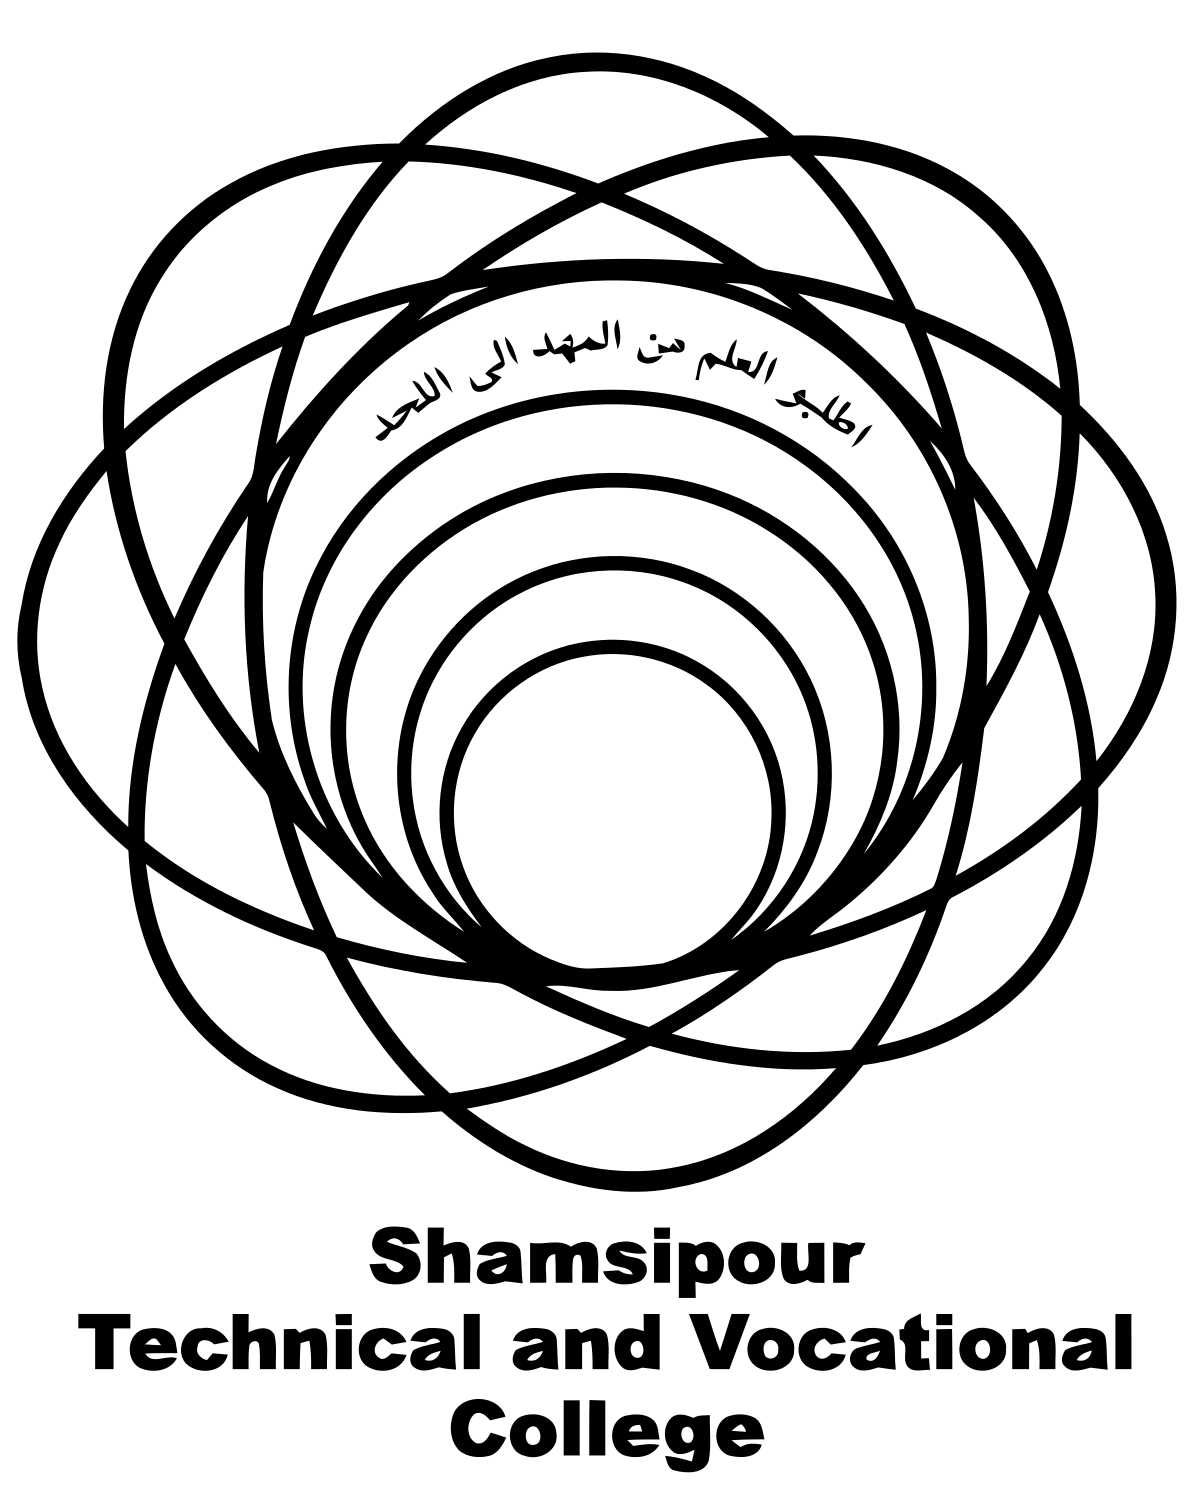
\includegraphics[width=1.1cm]{tvu.png}
  \end{minipage}%
  \hfill%
  \begin{minipage}{0.9\textwidth}\raggedleft
  دانشکده شمسی پور\\
  گزارش پروژه نهایی درس مباحث ویژه در برنامه نویسی\\
  \end{minipage}

\par\noindent\rule{\textwidth}{3pt}
{\par\centering\large گزارش \par}
{\par\centering\large پروژه چت چند وجهی مبتنی بر پروتکل ساکت در وب  \par}
\par\noindent\rule{\textwidth}{1pt}

\section{مقدمه}

  تمامی موارد صورت گرفته در قسمت سمت سرور، به لطف وجود پلتفرم قدرمتند    
\lr{Node.js}
با استفاده از کتابخانه و فریمورک
\lr{Express}
صورت گرفته است.
در این پروژه علاوه بر پروتکل 
\lr{HTTP}
برای ارتباط بلادرنگ
\footnote{RealTime}
از پروتکل وب سوکت
\footnote{Socket}
و از کتابخانه و فریمورک 
\lr{Socket.io}
مورد استفاده قرار گرفته است.

لازم به ذکر است که تمامی موارد سمت کاربر از تکنولوژی خاصی استفاده نشده است، بلکه
خیلی به صورت ساده از ساختار
\lr{HTML}
استفاده شده.



\section{HTTP 2 Web Socket}
در این پروژه برای داشتن ارتباط بلادرنگ در یک زمان
و داشتن وضعیت پایدار، سعی شده اکه از پروتکل
\lr{HTTP}
نمونه ای گرفته شده به سمت پروتکل وب سوکت انجام شده بطوری که 
بیشتر در مورد 
\lr{NameSpcase} ها
و 
\lr{Endpoint}
هایی که قرار است کاربران در آن به گفت و گو بپردازند، بحث شده.

ارتباطات دیگر به صورت حالت
\lr{HTTP}
که در آن در مورد 
در خواست ها
\lr{Requests}
و پاسخ دهی
\lr{Response}
نمی باشد.
بلکه برای ارسال اطلاعات چه از سمت کاربر چه از سمت سرور با استفاده از
فریمورک ساکت ای او، از دستور on برای گرفتن اطالاعات
و از دستوری به نام emit برای ارسال اطلاعات استفاده شده است.


\section{توضیح مختصر در رابطه با پروژه}
در این پروژه یکسری از فضاهایی وجود دارد که در آن کلاس ها وموضوع های 
مختلفی برای گفت و گو کردن وجود دارد، و کاربران به اختیار خودشان میتوانند وارد این 
فضاها شده و کلاس مربوط به خود را استفاده و در آن بحث کنند.

در این پروژه سعی شده تا از فضانام های ساده ای مانند.
\lr{Mozila}, \lr{Linux}, \lr{Wikipedia}
وجود دارد، که برای مثلا در قسمت موزیلا بحث هایی در مورد فضای اینترنتی و فضای مجازی
شده، یا مثلا در قسمت لینوکس در مورد سیستم عامل
\lr{Mac os Big Sur}
یا در مورد 
\lr{Redhat}
صحبت های مختلفی شده است.

لازم به ذکر است که تمام گفت و گو ها بین کاربران تا زمانی که سرور خاموش نشود(نمیرد)
در یک آرایه خیلی ساده باقی خواهد ماند تا کاربران بتوانند از سوابق گفت وگو های 
خود یک پیش نمایش حدودی داشته باشند.

قسمت فضا ها و کلاس ها و ذخیره موقت پیام ها در آرایه کاملا به صورت شئ گرا انجام شده.

بطوری که در فایلی ساده در مورد فضاهای نام یک نمونه از کلاس مربوط به آن گرفته شده و 
به وسیله این نمونه فضای نام مربوطه به آرایه مربوط به آن اضافه شده. کلاس هاهم به همین ترتیب
صورت گرفته و در نهایت به عنوان آرایه ای داخل فضا ذخیره شده است.

در قسمت سرور در قسمت اصلی این اطلاعات مربوط به فضاها و کلاس ها سعی شده که یک رندر شود
و در قسمت کاربر به وسیله ارتباط سوکت ارسال شود، و در قسمت کاربر این اطلاعات on
شده و بعد از آن به لطف زبان JS
تمام فرایند ها در قسمت کاربر از صدا زدن تا ارسال و نمایش اطلاعات از سمت سرور به 
سمت کاربر صورت گرفته است.

نکته ای که باید توجه داشته باشیم آن است که پیام ها از نقطه ای به سمت سرور ارسال میشود
و آن پیام از سمت سرور به سمت کاربر دوباره هدایت میشود تا کاربر پیام خود را در 
کلاس مربوطه ببیند، این فرایند برای تمامی کاربران قابل مشاهده و انجام می باشد.

نکته بعدی آن است که کاربری که از کلاس میخواهد به کلاس دیگری برود، 
ابتدا از کلاس مربوطه تابع خروج یا 
\lr{Left()}
فراخوانی میشود و برای رفتن به کلاس جدید تابع 
\lr{Join()}
برای ورود به آن گفت و گو استفاده میشود.
دلیل این کار آن است که اگر کاربر از کلاسی لفت ندهد و وارد کلاس بعد جوین شود 
تمام پیام های او نه تنها برادکست خواهد شد بلکه تمام پیام هایی که در کلاس قبلی نوشته 
بوده در کلاس جدیدی که وارد شده اضافه می شود و به نوعی با تخریب و ریداندنسی رو به رو خواهیم شد.

نکته آخری که مربوط به بخش کاربر می باشد آن است که کاربر با کلیک بر روی هر کدام از
\lr{Namespace}
ها در حقیقت با استفاده از تابع 
io.emit()
متن آن فضایی که در آن قرار دارد به سمت سرور ارسال شده و سمت سرور به وسیله سوکت
داخلی آن فضا را گرفته و کلا های مربوط به آن را ارسال خواهد کرد و در سمت 
کاربر این کلاس ها دریافت خواهد شد و با 
\lr{Loop Event}
مناسبی تمام کلاس ها برای کاربران به نمایش گذاشته می شود.


\section{فراموش نشود}
در این پروژه هیچ گونه احراز هویتی خاصی با امنیت خاص ایجاد نشده، چرا که 
به دلیل فرآینده های زیاد و زمان کمی که در اختیار داشته ام قسمت چت بین کاربران
با دقت بالایی پیاده سازی شده و فقط قسمت احراز هویت آن صورت نگرفته، اما به لطف کتابخانه
\lr{Passport.js}
این احراز هویت میتواند صورت گیرد اما به دلیل فرایند های جاری پروژه تا همین قسمت به صورت
کامل انجام شده است.




\newpage
\section*{منابع}

\medskip

\small
\LTR 
\latin


You can click on my GitHub page[1] \href{https://github.com/Asncodes-80/Socket.io/tree/master/slack} to see all source of this project as 
Clone Slack base on Javascript with [2] \href{https://socket.io/} Socket.io 
and [3] \href{http://expressjs.com/}Express framework .


\end{document}